\documentclass[12pt,letterpaper]{article}
\usepackage{graphicx,textcomp}
\usepackage{natbib}
\usepackage{setspace}
\usepackage{fullpage}
\usepackage{color}
\usepackage[reqno]{amsmath}
\usepackage{amsthm}
\usepackage{fancyvrb}
\usepackage{amssymb,enumerate}
\usepackage[all]{xy}
\usepackage{endnotes}
\usepackage{lscape}
\newtheorem{com}{Comment}
\usepackage{float}
\usepackage{hyperref}
\newtheorem{lem} {Lemma}
\newtheorem{prop}{Proposition}
\newtheorem{thm}{Theorem}
\newtheorem{defn}{Definition}
\newtheorem{cor}{Corollary}
\newtheorem{obs}{Observation}
\usepackage[compact]{titlesec}
\usepackage{dcolumn}
\usepackage{tikz}
\usetikzlibrary{arrows}
\usepackage{multirow}
\usepackage{xcolor}
\newcolumntype{.}{D{.}{.}{-1}}
\newcolumntype{d}[1]{D{.}{.}{#1}}
\definecolor{light-gray}{gray}{0.65}
\usepackage{url}
\usepackage{listings}
\usepackage{color}

\definecolor{codegreen}{rgb}{0,0.6,0}
\definecolor{codegray}{rgb}{0.5,0.5,0.5}
\definecolor{codepurple}{rgb}{0.58,0,0.82}
\definecolor{backcolour}{rgb}{0.95,0.95,0.92}

\lstdefinestyle{mystyle}{
	backgroundcolor=\color{backcolour},   
	commentstyle=\color{codegreen},
	keywordstyle=\color{magenta},
	numberstyle=\tiny\color{codegray},
	stringstyle=\color{codepurple},
	basicstyle=\footnotesize,
	breakatwhitespace=false,         
	breaklines=true,                 
	captionpos=b,                    
	keepspaces=true,                 
	numbers=left,                    
	numbersep=5pt,                  
	showspaces=false,                
	showstringspaces=false,
	showtabs=false,                  
	tabsize=2
}
\lstset{style=mystyle}
\newcommand{\Sref}[1]{Section~\ref{#1}}
\newtheorem{hyp}{Hypothesis}

\title{Problem Set 1}
\date{Due: October 1, 2021}
\author{ Marcus Ó Faoláin, 16327268. Applied Stats/Quant Methods 1.}

\begin{document}
	\maketitle
	
	\section*{Instructions}
	\begin{itemize}
		\item Please show your work! You may lose points by simply writing in the answer. If the problem requires you to execute commands in \texttt{R}, please include the code you used to get your answers. Please also include the \texttt{.R} file that contains your code. If you are not sure if work needs to be shown for a particular problem, please ask.
		\item Your homework should be submitted electronically on GitHub in \texttt{.pdf} form.
		\item This problem set is due before 8:00 on Friday October 1, 2021. No late assignments will be accepted.
		\item Total available points for this homework is 100.
	\end{itemize}
	
	\vspace{1cm}
	\section*{Question 1 (50 points): Education}

A school counselor was curious about the average of IQ of the students in her school and took a random sample of 25 students' IQ scores. The following is the data set:\\
\vspace{.5cm}

\lstinputlisting[language=R, firstline=40, lastline=40]{PS01.R}  

\vspace{1cm}

\begin{enumerate}
	\item Find a 90\% confidence interval for the average student IQ in the school.\\
	
	\item Next, the school counselor was curious  whether  the average student IQ in her school is higher than the average IQ score (100) among all the schools in the country.\\ 
	
	\noindent Using the same sample, conduct the appropriate hypothesis test with $\alpha=0.05$.
\end{enumerate}

\noindent
\textbf{Question 1 Part 1:}
\\\vspace{.5cm}

\noindent 
Since n is less than 30, we must use a t-score instead of a Z score. As the confidence coefficient is 0.90, we are looking for a t-value corresponding with (1-0.90)/2 = 0.05 using one-tailed test scores or 0.1 for 
two-tailed test scores.\\\vspace{.5cm}

\noindent
Since degrees of freedom = (n-1), we calculate the degrees of freedom = (25-1)
df = 24. The T-value at these points is 1.711
\\\vspace{.5cm}

\noindent
We calculate the sample mean to be ¯x = 98.44.

\lstinputlisting[language=R, firstline=59, lastline=59]{PS01.R}  
\noindent
\\\vspace{.0cm}

\noindent
We create an empty vector to hold the demeaned sum of yn.

\lstinputlisting[language=R, firstline=62, lastline=62]{PS01.R}  
\noindent
\\\vspace{.0cm}

\noindent
We add the demeaned sum of each element of y to the demeaned sum y vector. This is yn minus the mean of y (98.44).

\lstinputlisting[language=R, firstline=67, lastline=69]{PS01.R}
\noindent
\\\vspace{.0cm}

\noindent
We calculate the Squared Error for each element of demeaned sum y by squaring each element.

\lstinputlisting[language=R, firstline=73, lastline=73]{PS01.R}
\noindent
\\\vspace{.0cm}

\noindent
We then find the sum of the elements of the vector. Sum = 4114.16.

\lstinputlisting[language=R, firstline=76, lastline=76]{PS01.R}
\noindent
\\\vspace{.0cm}

\noindent
We find the variance of y by dividing the sum of the squared errors of y by the number of elements minus 1. Variance = 171.4233.

\lstinputlisting[language=R, firstline=80, lastline=80]{PS01.R}
\noindent
\\\vspace{.0cm}

\noindent
We find the standard deviation by finding the square root of the variance. SD = 13.09287.

\lstinputlisting[language=R, firstline=84, lastline=84]{PS01.R}
\noindent
\\\vspace{.0cm}

\noindent
We calculate the standard error using by dividing the standard deviation by the square root of the number of elements in y. SE = 2.618575.

\lstinputlisting[language=R, firstline=88, lastline=88]{PS01.R}
\noindent
\\\vspace{.0cm}

\noindent
We now multiply the standard error by the t-value we found earlier = 4.480381.

\lstinputlisting[language=R, firstline=91, lastline=91]{PS01.R}
\noindent
\\\vspace{.0cm}

\noindent
We now find the lower limit and the upper limit for the confidence interval by subtracting t-by-se1 from the mean and by adding it to it.

\lstinputlisting[language=R, firstline=96, lastline=99]{PS01.R}
\noindent
\\\vspace{.0cm}

\noindent
We calculate that the confidence interval is [93.95962, 102.92038]
\\\vspace{.5cm}

\newpage
\noindent
\textbf{Question 1 Part 2. }
\\\vspace{.5cm}

\noindent
5 steps to Hypothesis testing
\\\vspace{.5cm}

\noindent
\textbf{Step 1:} Assumptions. Since n is greater than 30, we will use a t-test to test the hypotheses. According to the question, the data is a random sample
\\\vspace{.5cm}

\noindent
Because we want to know whether the mean of the average school student is higher than the average among all schools in the country, we will perform a one-tailed test.
\\\vspace{.5cm}

\noindent
\textbf{Step 2:} We set up our null and alternative hypotheses.
\\\vspace{.5cm}

\noindent
H0: µ is less than or equal to 100. 

\noindent
Null Hypothesis: The average IQ of the students in the school is less than or equal to 100

\lstinputlisting[language=R, firstline=119, lastline=119]{PS01.R}

\noindent
Ha: µ is greater than 100.  

\noindent
Alternative Hypothesis: The average IQ of the students in the school is greater than 100.

\lstinputlisting[language=R, firstline=122, lastline=122]{PS01.R}

\noindent
\textbf{Step 3:} We calculate a test statistic.

\noindent
Test statistic formula = (¯x-mu0)/(s/ the square root of n)

\lstinputlisting[language=R, firstline=129, lastline=130]{PS01.R}

\noindent
We calculate the test statistic to be -0.5957439. 
The degrees of freedom (df) are (n-1) = (25-1) = 24.
\\\vspace{.5cm}

\noindent
\textbf{Step 4} - we must calculate the p-value.
\\\vspace{.5cm}

\noindent
We use the following formula in R to compute the probability of this test statistic occuring with degrees of freedom = 24.

\lstinputlisting[language=R, firstline=140, lastline=141]{PS01.R}

\noindent
The p-value is equal to 0.2784617.
\\\vspace{.5cm}

\noindent
\textbf{Step 5:} Draw a conclusion
\\\vspace{.5cm}

\noindent
Since the p-value is greater than the alpha (0.2784617 is greater than 0.05), the result is not extreme enough to be statistically significant. There is not enough evidence allowing us to reject the null hypothesis and to accept the alternative hypothesis.
\\\vspace{.5cm}

\noindent
Therefore, the school counselor cannot conclude that the average student IQ in her school is higher than the average IQ score (100) among all the schools in the country.
\\\vspace{.5cm}

\newpage

	\section*{Question 2 (50 points): Political Economy}

\noindent Researchers are curious about what affects the amount of money communities spend on addressing homelessness. The following variables constitute our data set about social welfare expenditures in the USA. \\
\vspace{.5cm}


\begin{tabular}{r|l}
	\texttt{State} &\emph{50 states in US} \\
	\texttt{Y} & \emph{per capita expenditure on shelters/housing assistance in state}\\
	\texttt{X1} &\emph{per capita personal income in state} \\
	\texttt{X2} &  \emph{Number of residents per 100,000 that are "financially insecure" in state}\\
	\texttt{X3} &  \emph{Number of people per thousand residing in urban areas in state} \\
	\texttt{Region} &  \emph{1=Northeast, 2= North Central, 3= South, 4=West} \\
\end{tabular}

\vspace{.5cm}
\noindent Explore the \texttt{expenditure} data set and import data into \texttt{R}.
\vspace{.5cm}
\vspace{.5cm}
\begin{itemize}

\item
Please plot the relationships among \emph{Y}, \emph{X1}, \emph{X2}, and \emph{X3}? What are the correlations among them (you just need to describe the graph and the relationships among them)?
\vspace{.5cm}
\item
Please plot the relationship between \emph{Y} and \emph{Region}? On average, which region has the highest per capita expenditure on housing assistance?
\vspace{.5cm}
\item
Please plot the relationship between \emph{Y} and \emph{X1}? Describe this graph and the relationship. Reproduce the above graph including one more variable \emph{Region} and display different regions with different types of symbols and colors.
\end{itemize}

\newpage
\noindent
\textbf{Question 2 Part 1:}


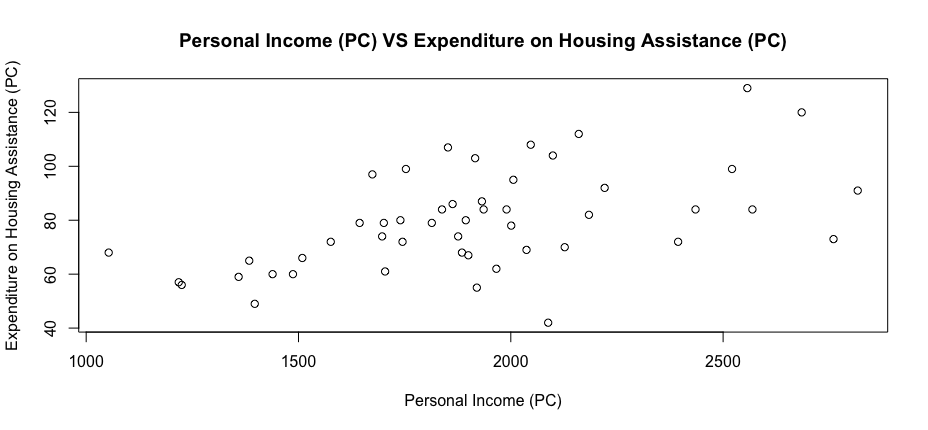
\includegraphics[width=150mm]{Rplot X1 against Y}

\noindent
The relationship between personal income per capita and expenditure on housing assistance per capita appears to be positively correlated. As one variable increases, so does the other. This means that states with higher personal income per capita also appear to have higher spending per capita on housing assistance.
\\\vspace{.5cm}

\lstinputlisting[language=R, firstline=171, lastline=175]{PS01.R}

\newpage

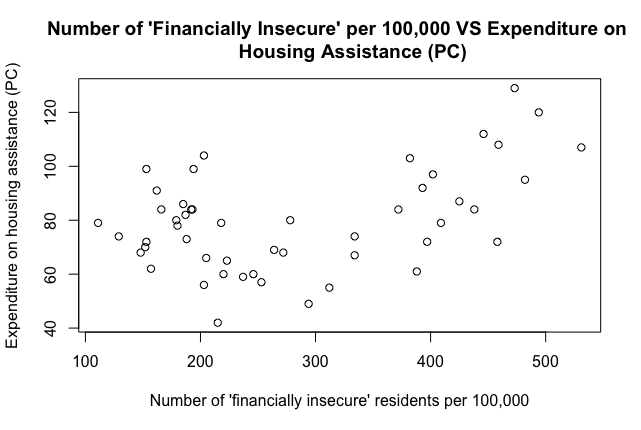
\includegraphics[width=150mm]{Rplot X2 against Y}

\noindent
The relationship between the number of 'financially insecure' residents per 100,000 and expenditure on housing assistance per capita appears to somewhat form a u-shaped curve. This would indicate a non linear relationship between the two variables, but rather a quadratic relationship. This would perhaps indicate that a squared function could describe the graph better than a linear one.
\\\vspace{.5cm}

\lstinputlisting[language=R, firstline=178, lastline=183]{PS01.R}

\newpage

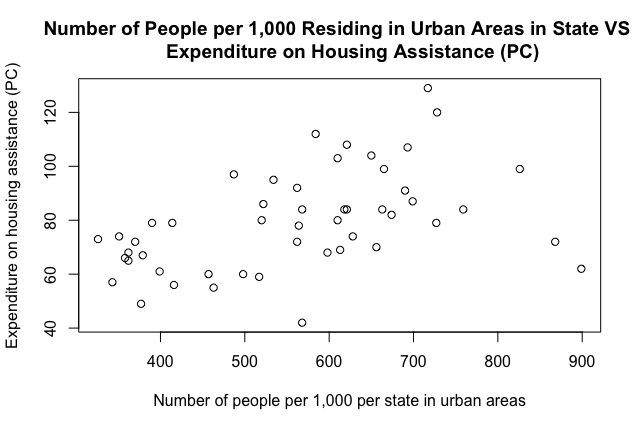
\includegraphics[width=150mm]{Rplot X3 against Y}

\noindent
The number of people residing in urban areas per thousand in the state appears to be somewhat positively correlated with expenditure on housing assistance, though it does not appear to be as strongly correlated as personal income per capita. 
States with a greater proportion of the population living in urban areas appear to in general have a greater amount of spending on housing assistance per capita.
\\\vspace{.5cm}

\lstinputlisting[language=R, firstline=186, lastline=191]{PS01.R}

\newpage

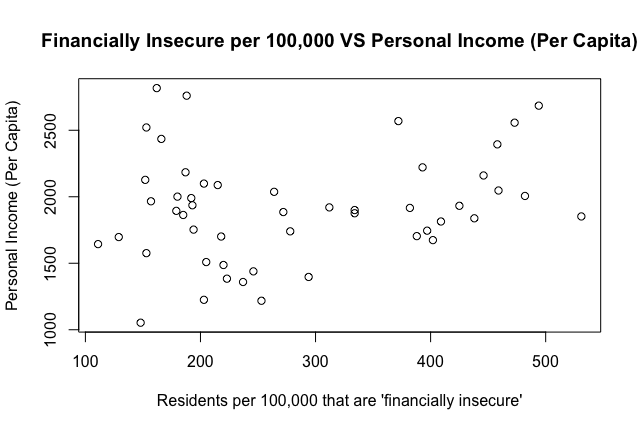
\includegraphics[width=150mm]{Rplot X2 against X1}

\noindent
There appears to be a weak relationship between the number of financially insecure' per 100,000 in the state and personal income per capita. They do not appear to be strongly correlated overall. There may however be a positive correlation between the two variables when the number of residents per 100,000 that are 'financially insecure' exceeds 400.
\\\vspace{.5cm}

\lstinputlisting[language=R, firstline=194, lastline=198]{PS01.R}

\newpage

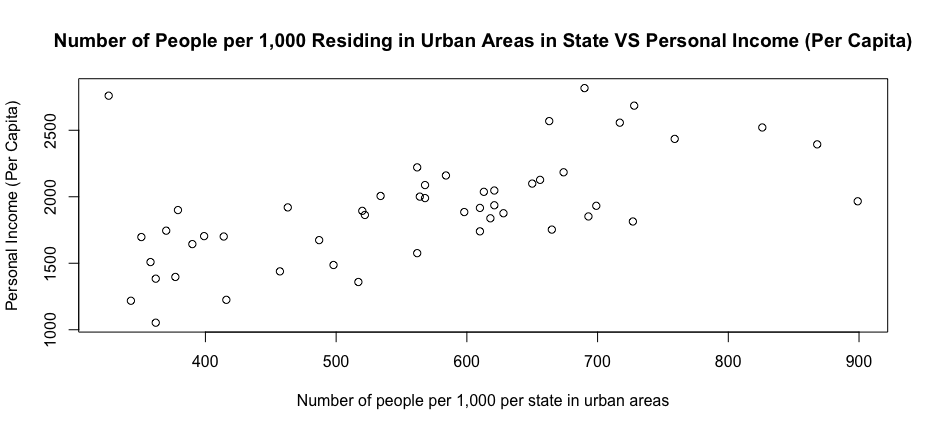
\includegraphics[width=150mm]{Rplot X3 against X1}

\noindent
There appears to be a very strongly positively correlated relationship between the number of people in urban areas per thousand in the state and the personal income per capita of the people in these states. As one of these variables goes up, it is very likely that the other will as well. This means that states with higher income per capita also have a higher proportion of people living in urban areas, though we do not have enough data yet to know whether one causes the other. 
\\\vspace{.5cm}

\lstinputlisting[language=R, firstline=201, lastline=205]{PS01.R}

\newpage

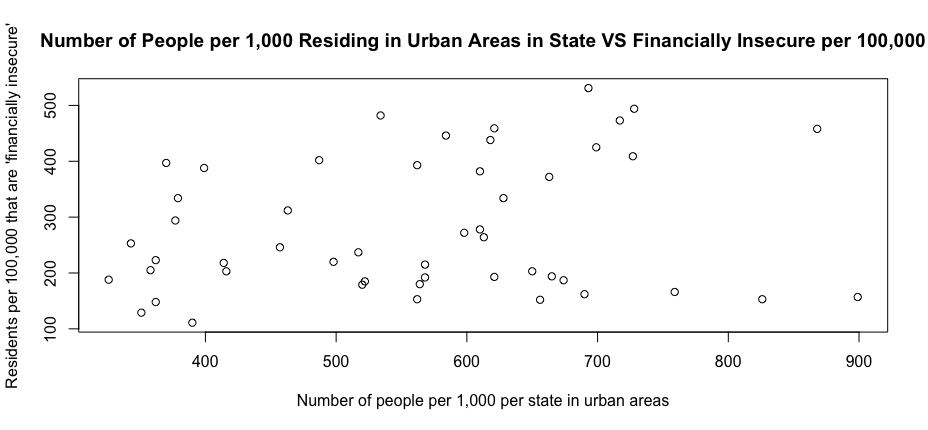
\includegraphics[width=150mm]{Rplot X3 against X2}

\noindent
At first glance, there does not appear to be any correlation between the number of people residing in urban areas per 1000 people in the state and the number of 'financially insecure' people per 100,000 in the state. The data points appear to be scattered around the plot without any clear relationship. The two variables seem to be neither positively nor negatively correlated.
\\\vspace{.5cm}

\lstinputlisting[language=R, firstline=208, lastline=212]{PS01.R}

\newpage

\noindent
\textbf{Question 2 Part 2:}


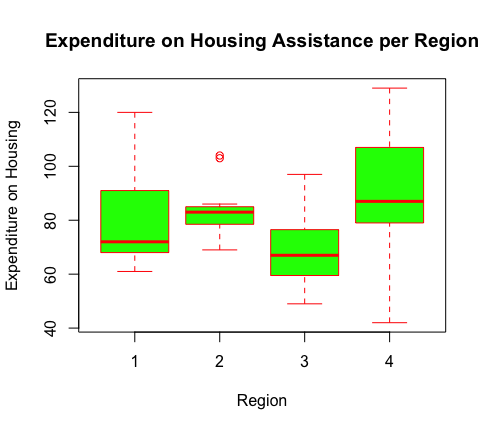
\includegraphics[width=150mm]{Rplot Housing Assistance per Region}

\noindent
On average, Region 4 (West) has the highest per capita expenditure on housing assistance. Its median, the red line in its box plot, is above that of all the others.
\\\vspace{.5cm}

\lstinputlisting[language=R, firstline=217, lastline=223]{PS01.R}

\newpage

\noindent
\textbf{Question 2 Part 3:}
\\\vspace{.5cm}

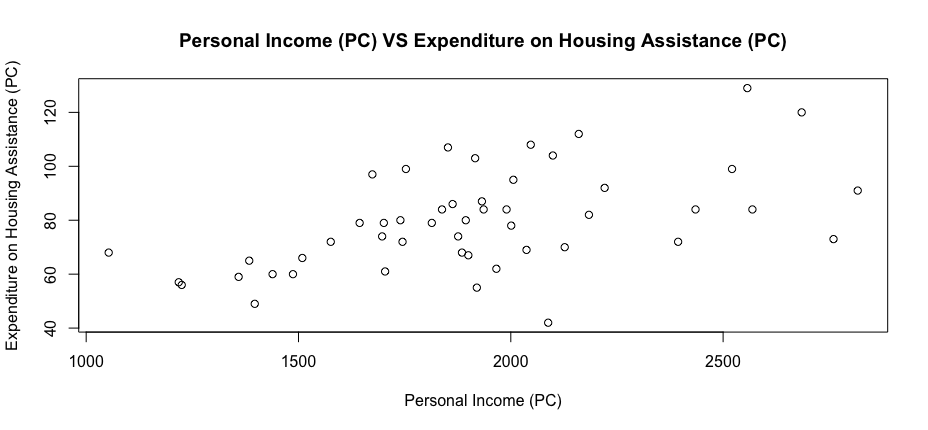
\includegraphics[width=150mm]{Rplot X1 against Y}

\noindent
The relationship between personal income per capita and expenditure on housing assistance per capita appears to be positively correlated. As one variable increases, so does the other. This means that states with higher personal income per capita also appear to have higher spending per capita on housing assistance.
\\\vspace{.5cm}

\lstinputlisting[language=R, firstline=229, lastline=233]{PS01.R}

\newpage

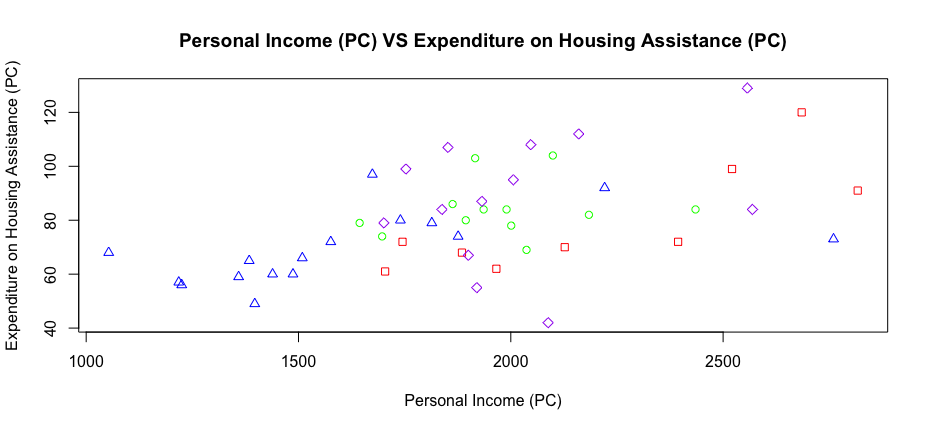
\includegraphics[width=150mm]{Rplot X1 against Y colours}

\noindent
We see the same graph here with each region represented by a different colour and and symbol. It is immediately noticeable that there is a grouping of blue triangles with low personal income per capita and low expenditure on housing assistance per capita. These blue triangles are all in the 'South' region.
\\\vspace{.5cm}

\noindent
1 = Northeast is represented by red squares, 2 = North Central is represented by green circles, 3 = South is represented by blue triangles and 4 = West is represented by purple diamonds.
\\\vspace{.5cm}

\lstinputlisting[language=R, firstline=243, lastline=250]{PS01.R}

\end{document}